\documentclass[11pt,twoside, openany]{extbook}
\input{preambule-prof}
  \addto\captionsfrench{%
    \renewcommand*{\contentsname}{ SÉQUENCE \No1 \vspace{0.2cm}\\ RÉCURRENCE ET\\ LIMITES DE SUITES}}

\begin{document}
%\chapter{\huge{RECURRENCE ET LIMITE DE SUITES}}
\tableofcontents 
\newpage
\myemptypage
%%%%%%%%%%%%%%%%%  TITRE  %%%%%%%%%%%%%%%%%%%%%%%%%%%%%
\tcbset{
         enhanced,
         colback=black!5!white,
         boxrule=0.1pt,
         colframe=black,
         fonttitle=\bfseries\large
        }
        \begin{tcolorbox}[    %%<<---- here
        lifted shadow={1mm}{-3mm}{5mm}{0.1mm}%
        {black!50!white}]
 \begin{center}
 {\textbf{\LARGE SEQUENCE \No1 \vspace{0.2cm}\\ \LARGE RÉCURRENCE ET LIMITES DE SUITES}}
 \end{center}
        \end{tcolorbox}
        \vskip0.5cm
%%%%%%%%%%%%%%%%%%%%%%%%%%%%%%%%%%%%%%%%%%%%%%%%%%%%%%%%%%%%%%%%%%%%

\section{PRINCIPE DE RÉCURRENCE}
	\begin{trm}[blue][Théorème : raisonnement par récurrence ]
		Soit $P(n)$ une propriété dépendant d'un entier naturel $n$. On suppose que : $P(n_0)$ est vraie.\\
        Pour tout entier naturel $n \ge n_0$ fixé, si $P(n)$ est vraie, et que $P(n+1)$ soit vraie, alors pour tout entier naturel $n$, $P(n)$ est vraie.
	\end{trm}

\medskip

\begin{tcolorbox}[colback= white, colframe=black!80, title= \section*{Méthode : Démonstration par récurrence}]
\begin{prop}[black][Méthode]
  Pour démontrer par récurrence qu'une propriété $P(n)$ est vraie pour tout entier naturel $n \ge n_0$, on procède en trois étapes.
\begin{itemize}
    \item \textbf{\ul{Étape $1$ : Initialisation}} \quad On vérifie que la propriété est vraie pour $n = n_0$.
    \item \textbf{\ul{ Étape $2$ : Hérédité }} \quad Soit $n$ un entier naturel tel que $n \ge n_0$.\\
On suppose que la propriété $P(n)$ est vraie (hypothèse de récurrence) et on démontre que $P(n + 1)$ est vraie.
    \item \textbf{\ul{ Étape $3$ : Conclusion }} On conclut que $P(n)$ est vraie pour tout entier naturel $n \ge n_0$
\end{itemize}  
\end{prop}
\noindent \textbf{\underline{Exemple 1}}\\
On considère la suite $(u_n)$ définie 
pour par $u_0=0$, puis pour tout entier $n$, $u_{n+1}=2+3u_n$.\\
Montrer que, pour tout entier $n$, $u_n=3^n-1$. 

\textcolor{blue}{\textbf{\underline{Correction :}}
%\vspace{0.3cm}
%\begin{center}
%\AffQuadrillage[NbCarreaux=30x16,Elargir=3/3]
%\AffQuadrillage[NbCarreaux=16x7,Elargir=2/2,Grille=Ruled,AffBarre=false]<gray!50!white>
%\end{center}
\begin{itemize}
    \item Initialisation : Vérifions que la propriété $P(n)$ est vraie pour  $n = 0$ :
$u_0 = 0 \quad \text{et} \quad 3^0 - 1 = 1 - 1 = 0$ \\
Ainsi, $u_0 = 3^0 - 1$ . La propriété $P(n)$ est vraie au rang  $0$ .
    \item Hérédité : Supposons que la propriété $P(n)$ est vraie $\forall n \geq 0$, c'est-à-dire que $u_n = 3^n - 1$, et montrons que $P(n+1)$ est vraie $\forall n \geq 0$, c'est-à-dire que $u_{n+1} = 3^{n+1} - 1$.\\
On sait que : $u_{n+1} = 2 + 3u_n$ ,  or $u_n = 3^n - 1$, $\iff u_{n+1} = 2 + 3(3^n - 1)= 2 + 3^{n+1} - 3$ \\ $\iff u_{n+1} = 3^{n+1} - 1$ \\
Ainsi, si la propriété est vraie pour $n$, elle est aussi vraie pour $n + 1$.
    \item Conclusion : Par le principe de récurrence, pour tout entier $n$, $u_n=3^n-1$.
\end{itemize}}
\end{tcolorbox}



\newpage
\begin{application}{}
. On considère la fonction définie sur $\R$ par $f(x)=\dfrac{1}{4}x^2-\dfrac{1}{2}x+\dfrac{5}{4}$ et la suite $(u_n)$ définie par $u_0 = 3$ et pour tout $n\in\N$, \quad $u_{n+1} = f(u_n)$. 
\begin{enumerate}
	\item Étudier le sens de variation de $f$ sur $[1\;;\;3]$.\vspace{0.5cm}  \\
    \textcolor{blue}{\begin{minipage}{8cm}
    Pour tout $x \in \R \quad f'(x)=\dfrac{1}{2}x-\dfrac{1}{2}$\\
    \medskip
 $f'(x)=0 \iff \dfrac{1}{2}x-\dfrac{1}{2}=0 \iff  x=1 $.\vspace{0.5em}\\ 
 On obtient le TV ci-contre. $f(1)=1$ et $f(3)=2$\\
 \medskip
 Sur $[1\;;\;3]$, la fonction $f$ est croissante.
\end{minipage} 
\hspace { 0,005 \textwidth }
\begin{minipage}{10cm} 
\begin{center}
  \begin{tikzpicture}[baseline, scale=0.6]
    \tkzTabInit[lgt=2.5,deltacl=0.7,espcl=2.3]{ $x$ / 1.5, $f^{\prime}(x)$ / 1.5, Variat* \\ de $f$ / 3}{ $-\infty$, $1$,  $ $, $+\infty$ }
	\tkzTabLine{, -,z,+,t,+,}
	\tkzTabVar{  +/$ $, -/$ 1$,R, +/$ $}
    \tkzTabVal[draw]{2}{4}{0.5}{3}{2}
	\end{tikzpicture}  
\end{center}
\end{minipage}\\}
	\item Démontrer par récurrence que, pour tout entier naturel $n$, $1 \leqslant u_n \leqslant 3$ \\
    \textcolor{blue}{
\begin{itemize}
    \item Initialisation : Vérifions que la propriété $P(n)$ est vraie pour  $n = 0$ :\\
$u_0 = 3$, on a bien $1 \leqslant u_0 \leqslant 3$.
La propriété $P(n)$ est vraie au rang  $0$ .
    \item Hérédité : Supposons que la propriété $P(n)$ est vraie $\forall n \in \N$, c'est-à-dire que $1 \leqslant u_n \leqslant 3$, et montrons que $P(n+1)$ est vraie $\forall n \in \N$, c'est-à-dire que $1 \leqslant u_{n+1} \leqslant 3$.\\
On sait que : $1 \leqslant u_n \leqslant 3$ ,  or sur $[1\;;\;3]$, la fonction $f$ est croissante. \\ Alors $ f(1) \leqslant f(u_n) \leqslant f(3) \iff 1 \leqslant u_{n+1} \leqslant 2 \leqslant 3 \iff 1 \leqslant u_{n+1} \leqslant 3$ \\
Ainsi, si la propriété est vraie pour $n$, elle est aussi vraie pour $n + 1$.
    \item Conclusion : Par le principe de récurrence, pour tout entier $n \in \N$, $1 \leqslant u_n \leqslant 3$.
\end{itemize}} \vspace{0.5cm}
	\item Démontrer que la suite $(u_n)$ est décroissante. \vspace{0.5cm}\\
     \textcolor{blue}{$(u_n)$ décroissante $\iff \forall n \in \N$ : $u_{n+1} \leqslant u_n \quad : P(n) $. 
\begin{itemize}
    \item Initialisation : Vérifions que la propriété $P(n)$ est vraie pour  $n = 0$ :\\
$u_0 = 3$, on a bien $1 \leqslant u_0 \leqslant 3$.
La propriété $P(n)$ est vraie au rang  $0$ .
    \item Hérédité : Supposons que la propriété $P(n)$ est vraie $\forall n \in \N$, c'est-à-dire que $u_{n+1} \leqslant u_n$, et montrons que $P(n+1)$ est vraie $\forall n \in \N$, c'est-à-dire que $u_{n+2} \leqslant u_{n+1}$.\\
On sait que : $u_{n+1} \leqslant u_n$ ,  or sur $[1\;;\;3]$, la fonction $f$ est croissante. \\ Alors $ f(u_{n+1}) \leqslant f(u_n)  \iff u_{n+2} \leqslant u_{n+1}$ \\
Ainsi, si la propriété est vraie pour $n$, elle est aussi vraie pour $n + 1$.
    \item Conclusion : Par le principe de récurrence, pour tout entier $n \in \N$, $u_{n+1} \leqslant u_n$.
\end{itemize}}
\end{enumerate}
\end{application}







\newpage
\section{LIMITE D'UNE SUITE}

\subsection{Limite finie et limite infinie}

\begin{defi}[Green][Définition : limite finie et suite convergente]
La suite numérique $(u_n)$ est \textbf{convergente} si ses termes se rapprochent de plus en plus d'un nombre fixe $\ell$ (appelé limite finie) lorsque $n$ devient très, très grand.
\center \fcolorbox{Green}{green!30!}{\text{On note:}\textbf{$\lim\limits_{n \rightarrow +\infty} u_n=\ell$}}  
\end{defi}

\medskip
\noindent \textbf{\ul{Exemple:}}\\ Soit la suite $(u_n)$ définie pour $n\geqslant 1$ par $u_n=\dfrac{1}{n}+1$. Le tableau de valeur ci-dessous nous donne les valeurs de $u_n$ pour des valeurs de $n$ croissantes.
\begin{center}
{\renewcommand{\arraystretch}{0.9} %donne la distance entre les lignes%
{\setlength{\tabcolsep}{0.53cm} %donne la distance entre les collones%
    \begin{tabular}{|c|c|c|c|c|c|c|c|c|}
\hline
$n$   & 1 & 2   & 7    & 10  & 50   & 100  & 1000  & $10^7$ \\ \hline
$u_n$ & 2 & 1,5 & 1,14 & 1,1 & 1,02 & 1,01 & 1,001 & 1,0000001 \\ \hline
\end{tabular}}} 
\end{center}
Pour $n$ aussi grand, $u_n$ se rapproche de $1$, on dit alors que $\lim\limits_{x \rightarrow +\infty} u_n= \lim\limits_{x \rightarrow +\infty} \dfrac{1}{n}+1 =1$

\begin{defi}[Green][Définition : limite infinie et suite divergente]
\begin{itemize}
    \item [$\bullet$] On dit qu'une suite $(u_n)$ a pour limite $+\infty$ (respectivement $-\infty$)  quand $n$ tend vers $+\infty$ (respectivement $-\infty$) lorsque, quel que soit le réel $A$, on a $u_n>A$ (respectivement $u_n<A$) à partir d'un certain rang. Une telle suite est dite \textbf{divergente}.\\
    \hspace*{2cm}\fcolorbox{Green}{green!30!}{\text{ On note:} $\lim\limits_{n \rightarrow +\infty} u_n= +\infty$ (\text{respectivement} $\lim\limits_{n \rightarrow +\infty} u_n=-\infty$)} 
    \item[$\bullet$] Une suite peut diverger sans pour autant tendre vers $\pm\infty$, si elle n'a pas de limite.  
\end{itemize}
\end{defi}

\medskip


\noindent \textbf{\ul{Exemple 1:}}\\ Soit la suite $(u_n)$ définie pour $n\geqslant 1$ par $u_n=n^2$. Le tableau de valeur ci-dessous nous donne les valeurs de $u_n$ pour des valeurs de $n$ croissantes.
\begin{center}
{\renewcommand{\arraystretch}{0.9} %donne la distance entre les lignes%
{\setlength{\tabcolsep}{0.6cm} %donne la distance entre les collones%
    \begin{tabular}{|c|c|c|c|c|c|c|c|c|}
\hline
$n$   & 1 & 2   & 7    & 10  & 50   & 100  & 1000  & $10^7$ \\ \hline
$u_n$ & 1 & 4 & 49 & 100 & 2500 & $10^4$ & $10^6$ & $10^{14}$ \\ \hline
\end{tabular}}} 
\end{center}
Pour $n$ aussi grand, $u_n$ se rapproche de $+\infty$, on dit alors que $\lim\limits_{n \rightarrow +\infty} u_n= \lim\limits_{n \rightarrow +\infty} n^2 =+\infty$\\
\medskip
\textbf{\ul{Exemple 2:}}\\La suite $(u_n)$ définie pour tout $n\in \mathbb{N}$ par $u_n=(-1)^n$ n'a pas de limite. On a deux cas :
\begin{multicols}{2}
   \begin{itemize}
\item si $n$ est pair, $u_n=1$ ;
\item si $n$ est impair, $u_n=-1$.
\end{itemize} 
\end{multicols}
La suite $(u_n)$ oscille constamment entre les valeurs $-1$ et $1$, elle ne converge pas vers une valeur fixe, elle est alors divergente.

\subsection{Limites de suites usuelles}
\begin{propa}
\begin{itemize}
    %\item Les suites de terme général $\sqrt{n}$, $n$, $n^2$, $n^3$ et, plus généralement, $n^k$ avec $k\in\mathbb{N}^*$  divergent vers $+\infty$.
   \item[$\bullet$]  $\displaystyle \lim_{n\rightarrow +\infty} \sqrt{n}=+\infty$, $\displaystyle \lim_{n\rightarrow +\infty} n=+\infty$, $\displaystyle \lim_{n\rightarrow +\infty} n^2=+\infty$, $\displaystyle \lim_{n\rightarrow +\infty} n^3=+\infty$ \vspace{0.5em} \\ \hspace*{2cm} 
    et, plus généralement, \fcolorbox{red}{red!20!}{$\displaystyle \lim_{n\rightarrow +\infty} n^k=+\infty$} pour $k\in\mathbb{N}^*$.
  %\item Les suites de terme général $\dfrac{1}{\sqrt{n}}$, $\dfrac{1}{n}$, $\dfrac{1}{n^2}$, $\dfrac{1}{n^3}$ et, plus généralement, $\dfrac{1}{n^k}=n^{-k}$ avec $k\in\mathbb{N}^*$  convergent vers $0$.
   \item[$\bullet$]  $\displaystyle \lim_{n\rightarrow +\infty} \dfrac{1}{\sqrt{n}}=0$, $\displaystyle \lim_{n\rightarrow +\infty} \dfrac{1}{n}=0$, $\displaystyle \lim_{n\rightarrow +\infty} \dfrac{1}{n^2}=0$, $\displaystyle \lim_{n\rightarrow +\infty} \dfrac{1}{n^3}=0$ \vspace{0.5em} \\  \vspace{0.5em} \hspace*{2cm} et, plus généralement, \fcolorbox{red}{red!20!}{$\displaystyle \lim_{n\rightarrow +\infty} \dfrac{1}{n^k}=0$} pour $k\in\mathbb{N}^*$.
   \item[$\bullet$]  La suite de terme général $q^n$ converge vers $0$ si $-1<q<1$.
        \begin{itemize}
           \item converge vers $0$ si $-1<q<1$ ;
           \item diverge vers $+\infty$ si $q>1$ ;
           \item n'a pas de limite si $q\leqslant -1$.
        \end{itemize}  
  \end{itemize}

\end{propa}


\section{CALCUL DE LIMITES D'UNE SUITE}
\subsection{Utiliser les propriétés opératoires sur les limites}

\noindent Tous les résultats suivants sont admis.  Soient $(u_n)$ et $(v_n)$ deux suites convergentes ou divergeant vers l'infini. Soient $\ell_1$ et $\ell_2$ deux nombres réels. 
\subsubsection{Limite de la somme $u_n+v_n$}
\begin{center}
{\renewcommand{\arraystretch}{1.2} %donne la distance entre les lignes%
{\setlength{\tabcolsep}{0.6cm} %donne la distance entre les collones%
\begin{tabular}{|r|*5{c|}>{\columncolor[RGB]{211, 211, 211}}c|}
\hline
$\lim\limits_{n \rightarrow +\infty}  u_n$ & \multicolumn{3}{c|}{$\ell_1$} & $+\infty$ & $-\infty$ & $+\infty$\\
\hline
$\lim\limits_{n \rightarrow +\infty}  v_n$ & $\ell_2$ & $+\infty$ & $-\infty$ & $+\infty$ & $-\infty$ & $-\infty$\\
\hline
\hline
$\lim\limits_{n \rightarrow +\infty}  (u_n+v_n)$ & $\ell_1+\ell_2$ & $+\infty$ & $-\infty$ & $+\infty$ & $-\infty$ & F.I.\\
\hline
\end{tabular}}}
\end{center}

\begin{Remarque}
    .F.I. signifie \og Forme Indéterminée \fg{}. On ne peut pas conclure le calcul de limite : tous les résultats sont possibles. Voici trois exemples où $\lim\limits_{n \rightarrow +\infty}u_n=+\infty$ et $\lim\limits_{n \rightarrow +\infty} v_n=-\infty$ donnent trois résultats différents : 

\begin{enumerate}
\item Si $u_n= 2n$ et $v_n=-n$.\quad On a \quad $u_n+v_n= n$ \quad donc \quad $\lim\limits_{n \rightarrow +\infty} u_n + v_n =+\infty$.\vspace{0.5em}
\item Si $u_n= n$ et $v_n=-n$.\quad On a \quad $u_n+v_n=0$ \quad donc \quad $\lim\limits_{n \rightarrow +\infty} u_n + v_n =0$.\vspace{0.5em}
\item Si $u_n=n$ et $v_n=-2n$.\quad On a \quad $u_n+v_n=-n$ \quad donc \quad $\lim\limits_{n \rightarrow +\infty} u_n + v_n =-\infty$.\vspace{0.5em}
\item Si $u_n=n^2$ et $v_n=-n^3$.\quad On a \quad $u_n+v_n=n^2-n^3$ \quad donc \quad $\lim\limits_{n \rightarrow +\infty} u_n + v_n =-\infty$.
\end{enumerate}
\end{Remarque}
\newpage
\textbf{\ul{Exemple:}}
Soit $(u_n)$ la suite définie sur $\N^*$ par 
$u_n=n^3+\dfrac{e}{3}-5$. 
\begin{equation*}
	\left.
	\begin{aligned}
		 \lim\limits_{n \rightarrow +\infty} n^3 &= +\infty \quad \\
		\lim\limits_{n \rightarrow +\infty} \dfrac{e}{3}-5 &= \dfrac{e}{3}-5 \quad
	\end{aligned}
	\right\}
	\quad \text{Par addition des limites $\lim\limits_{n \rightarrow +\infty} n^3+\dfrac{e}{3}-5=+\infty$}
\end{equation*}
\subsubsection{Limite du produit $u_n \times v_n$}

{\renewcommand{\arraystretch}{1.2} %donne la distance entre les lignes%
{\setlength{\tabcolsep}{0.4cm} %donne la distance entre les collones%
\begin{tabular}{|l||*{8}{c|}>{\columncolor[RGB]{211, 211, 211}}c|}\hline
$\lim\limits_{n \rightarrow +\infty} u_n$ & $\ell_1$ & \multicolumn{2}{c|}{$\ell_1>0$} & \multicolumn{2}{c|}{$\ell_1<0$} & \multicolumn{2}{c|}{$+\infty$} & $-\infty$ & $0$\\
\hline
$\lim\limits_{n \rightarrow +\infty} v_n$  & $\ell_2$ & $+\infty$ & $-\infty$ & $+\infty$ & $-\infty$ & $+\infty$ & $-\infty$ & $-\infty$ & $\pm\infty$\\
\hline
\hline
$\lim\limits_{n \rightarrow +\infty} (u_n\times v_n)$ & $\ell_1\times\ell_2$ & $+\infty$ & $-\infty$ & $-\infty$ & $+\infty$ & $+\infty$ & $-\infty$ & $+\infty$ & F.I. \\
\hline
\end{tabular}}}\\

\textbf{\ul{Exemple 1:}}\\
Soit $(u_n)$ la suite définie sur $\N$ par $u_n=-5n^2 \sqrt{n}$. 
\begin{equation*}
	\left.
	\begin{aligned}
		\lim\limits_{n \rightarrow +\infty} 5n^2 &= +\infty \quad \\
		\lim\limits_{n \rightarrow +\infty}  \sqrt{n} &= +\infty 
	\end{aligned}
	\right\}
	\quad \text{Par produit des limites $\lim\limits_{n \rightarrow +\infty} 5n^2 \sqrt{n}=+\infty$}
\end{equation*}

\noindent \textbf{\ul{Exemple 2:}}\\
Soit $(u_n)$ la suite définie sur $\N$ par $u_n=(2-n)(n^2+3)$. 
\begin{equation*}
	\left.
	\begin{aligned}
		\lim\limits_{n \rightarrow +\infty} 2-n &= -\infty \quad \\
		\lim\limits_{n \rightarrow +\infty} n^2+3 &= +\infty 
	\end{aligned}
	\right\}
	\quad \text{Par produit des limites $\lim\limits_{n \rightarrow +\infty} (2-n)(n^2+3)=-\infty$}
\end{equation*}
\subsubsection{Limite du quotient $\dfrac{u_n}{v_n}$}
Dans les tableaux suivants :
\begin{itemize}
\item $0^+$ et $0^-$ désignent des convergences vers 0 par valeurs positives et  par valeurs négatives.
\end{itemize}

{\renewcommand{\arraystretch}{1.5} %donne la distance entre les lignes%
{\setlength{\tabcolsep}{0.15cm} %donne la distance entre les collones%
\begin{tabular}{|l||*{8}{c|}*{2}{>{\columncolor[RGB]{211, 211, 211}}c|}}
\hline
$\lim\limits_{n \rightarrow +\infty} u_n$ & \multicolumn{2}{c|}{$\ell_1$} & \multicolumn{2}{c|}{$+\infty$} & \multicolumn{2}{c|}{$-\infty$}  & $\ell_1>0$ ou $+\infty$ & $\ell_1<0$ ou $-\infty$ & $0$& $\pm\infty$\\
\hline
$\lim\limits_{n \rightarrow +\infty} v_n$ & $\ell_2\neq 0$ & $\pm\infty$ & $\ell_2>0$ & $\ell_2<0$ & $\ell_2>0$ & $\ell_2<0$  & $0^\pm$ & $0^\pm$ & 0 & $\pm\infty$\\
\hline
\hline
$\lim\limits_{n \rightarrow +\infty} \dfrac{u_n}{v_n}$ & $\dfrac{\ell_1}{\ell_2}$ & $0$ & $+\infty$ & $-\infty$ & $-\infty$ & $+\infty$  & $\pm\infty$ & $\mp\infty$ & F.I.& F.I. \\
\hline
\end{tabular}}}\\

\noindent \textbf{\ul{Exemple :}}\\
Soit $(u_n)$ la suite définie sur $\N^*$ par $u_n=\dfrac{2+\dfrac{3}{n}}{n^2+\sqrt{n}}$. 
\begin{equation*}
	\left.
	\begin{aligned}
		\lim\limits_{n \rightarrow +\infty} 2+\dfrac{3}{n} &= 2 \quad \\
		\lim\limits_{n \rightarrow +\infty}  n^2+\sqrt{n} &= +\infty 
	\end{aligned}
	\right\}
	\quad \text{Par quotient des limites $\lim\limits_{n \rightarrow +\infty} \dfrac{2+\dfrac{3}{n}}{n^2+\sqrt{n}}=0$}
\end{equation*}
\newpage
\subsection{Cas des formes indéterminées }
\selectlanguage{english}
On peut reconnaître les formes indéterminées pour lesquelles il faudra utiliser des calculs algébriques ou utiliser d'autres propriétés sur les calculs de limites afin de \textbf{lever l'indétermination}.\\ Les quatre formes indéterminées sont, par abus d'écriture : \enquote{$\dfrac{\infty}{\infty}$} \,;\,\enquote{$\infty-\infty$} \,;\,\enquote{$0 \times \infty$} \,et\;\enquote{$\dfrac{0}{0}$}.

\begin{tcolorbox}[colback= white, colframe=black!80, title= \section*{Méthode : Lever l’indétermination pour un polynôme}]
\begin{prop}[black][]
Pour un polynôme ou un quotient de polynômes, on lève l'indétermination en factorisant par \textbf{le monôme le plus haut degré}.
\end{prop}
\noindent \textbf{\ul{Exemple 1 :}}\\
soit la suite $(u_n)$ définie sur $\N$ par $u_n=n^2-2n+4$. 
\begin{equation*}
	\left.
	\begin{aligned}
		\lim\limits_{n \rightarrow +\infty} n^2 &= +\infty \quad \\
		\lim\limits_{n \rightarrow +\infty}  -2n+4 &= -\infty 
	\end{aligned}
	\right\}
	\quad \text{Par somme des limites, on obtient la forme indéterminée : $\infty-\infty$}
\end{equation*}
Levons l’indétermination en factorisant : 
\begin{align*}
    u_n&=n^2-2n+4 = n^2\left(1-\dfrac{2n}{n^2}+\dfrac{4}{n^2}\right)= n^2\left(1-\dfrac{2}{n}+\dfrac{4}{n^2}\right)
\end{align*}
\begin{equation*}
	\left.
	\begin{aligned}
		\lim\limits_{n \rightarrow +\infty} n^2 &= +\infty \quad \\
		\lim\limits_{n \rightarrow +\infty}  1-\dfrac{2}{n}+\dfrac{4}{n^2} &= +\infty
	\end{aligned}
	\right\}
	\quad \text{Par produit des limites,$\lim\limits_{n \rightarrow +\infty} n^2\left(1-\dfrac{2}{n}+\dfrac{4}{n^2}\right)=\lim\limits_{n \rightarrow +\infty}u_n=+\infty$}
\end{equation*}

 \noindent \textbf{\ul{Exemple 2 :}}\\
soit la suite $(u_n)$ définie sur $\N$ par $v_n=\dfrac{n^2+3n-5}{n^3-6n^2+1}$. \\
Le numérateur et le dénominateur sont des polynômes qui vont tendre vers $\pm\infty$.\\ On obtiendra alors une forme indéterminée du type : \enquote{$\dfrac{\infty}{\infty}$}\\
Levons l’indétermination en factorisant :\vspace{0.5em}
\begin{align*}
    v_n&=\dfrac{n^2+3n-5}{n^3-6n^2+1}\\&=\dfrac{n^2\left(1-\dfrac{3n}{n^2}-\dfrac{5}{n^2}\right)}{n^3\left(1-\dfrac{6n^2}{n^3}+\dfrac{1}{n^3}\right)} = \dfrac{\left(1-\dfrac{3}{n}-\dfrac{5}{n^2}\right)}{n\left(1-\dfrac{6}{n}+\dfrac{1}{n^3}\right)} 
\end{align*}

\begin{equation*}
	\left.
	\begin{aligned}
		\lim\limits_{n \rightarrow +\infty} 1-\dfrac{3}{n}-\dfrac{5}{n^2} &= 1 \quad \\
		\lim\limits_{n \rightarrow +\infty} n\left(1-\dfrac{6}{n}+\dfrac{1}{n^3}\right) &= +\infty \times 1= +\infty 
	\end{aligned}
	\right\}
	\quad \text{Par quotient des limites,$\lim\limits_{n \rightarrow +\infty}u_n=0$}
\end{equation*}

\end{tcolorbox}









\newpage
\noindent
\ul{\bf Méthode en cas de forme indéterminée: différence de racines carrées} \\ On lève l'indétermination en multipliant par le conjugué de l'expression.
\\
\noindent \textbf{\ul{Exemple :}}\\soit la suite $(u_n)$ définie sur $\N$ par $v_n= \sqrt{n^2+1}-\sqrt{n^2-3}$. \\
Les deux termes ont comme limite $+\infty$.\\ On obtiendra alors une forme indéterminée du type : \enquote{$+\infty-\infty$}\\
Levons l’indétermination :\vspace{0.5em}
\begin{align*}
v_n&= \sqrt{n^2+1}-\sqrt{n^2-3}
=\left(\sqrt{n^2+1}-\sqrt{n^2-3}\right) \times \dfrac{\left(\sqrt{n^2+1}+\sqrt{n^2-3}\right)}{\left(\sqrt{n^2+1}+\sqrt{n^2-3}\right)}\\
&= \dfrac{\left(\sqrt{n^2+1}-\sqrt{n^2-3}\right)\left(\sqrt{n^2+1}+\sqrt{n^2-3}\right)}{\left(\sqrt{n^2+1}+\sqrt{n^2-3}\right)}
\\&=\dfrac{\left(\sqrt{n^2+1}\right)^2-\left(\sqrt{n^2-3}\right)^2}{\left(\sqrt{n^2+1}+\sqrt{n^2-3}\right)}\\
&=\dfrac{\left(n^2+1\right)-\left(n^2-3\right)}{\left(\sqrt{n^2+1}+\sqrt{n^2-3}\right)}
=\dfrac{n^2+1-n^2+3}{\sqrt{n^2+1}+\sqrt{n^2-3}}
\\&=\dfrac{4}{\sqrt{n^2+1}+\sqrt{n^2-3}}
\end{align*}
\begin{equation*}
	\left.
	\begin{aligned}
		\lim\limits_{n \rightarrow +\infty}4 &= 4 \quad \\
		\lim\limits_{n \rightarrow +\infty}\sqrt{n^2+1}+\sqrt{n^2-3} &= +\infty 
	\end{aligned}
	\right\}
	\quad \text{Par quotient des limites,$\lim\limits_{n \rightarrow +\infty}v_n=0$}
\end{equation*}

\subsection{Cas de la suite {\boldmath $(q^n)$}}
\begin{prop}[Red][Propriété : limites et suite géométrique (admise)]
Soit $q$ un nombre réel.
\begin{itemize}
\item Si $q<-1$ alors la limite n'existe pas et la suite $(q^n)$ diverge.
\item Si $-1<q<1$ alors la suite $(q^n)$ converge vers 0.
\item Si $q=1$ la suite $(q^n)$ est constante et converge vers 1. 
\item Si $q>1$ alors la suite $(q^n)$ tend vers $+\infty$.
\end{itemize}
\end{prop}
\medskip
 \noindent \textbf{\ul{Exemple :}}\\
Déterminer les limites des suites suivantes (si elles existent). 
\begin{multicols}{2}
\begin{enumerate}
\item $u_n= -0,5\times (1,2)^n$ \vspace{0.6em}\\  $\lim\limits_{n \rightarrow +\infty}u_n=-0,5 \times +\infty = -\infty$ .
\item $v_n=\dfrac{4}{5}\left(\dfrac{9}{10}\right)^n-6$ \vspace{0.6em}\\  $\lim\limits_{n \rightarrow +\infty}v_n=0-6=-6$.
\end{enumerate}
\end{multicols}
$3.$ $w_n=(-4)^n$ la limite n'existe pas car $q=-4<-1$.







\section{Limites et comparaison }
\begin{trm}[blue][Théorème de comparaison : limites infinies (admis)]
    Soient $(u_n)$ et $(v_n)$ deux suites telles que, à partir d'un certain rang, $u_n \leqslant v_n$.
\begin{enumerate}
\item Si $\displaystyle \lim_{n \to +\infty} u_n=+\infty$ alors $\displaystyle \lim_{n \to +\infty} v_n=+\infty$.\vspace{0.5em}
\item Si $\displaystyle \lim_{n \to +\infty} v_n=-\infty$ alors $\displaystyle \lim_{n \to +\infty} u_n=-\infty$.\vspace{0.5em}
\item Si $\displaystyle \lim_{n \to +\infty} u_n=\ell_1$ et $\displaystyle \lim_{n \to +\infty} v_n=\ell_2$  alors $\ell_1\leqslant\ell_2$.
\end{enumerate}
\end{trm}

\medskip
 \noindent \textbf{\ul{Exemple :}}\\
 soit la suite $(u_n)$ définie sur $\N$ par $n^2+(-1)^n$.\\
 On va comparer cette suite avec une autre suite dont on peut determiner facilement sa limite en $+\infty$.
 On sait que pour tout $n \in \N$, $(-1)^n \geq -1 \iff n^2+(-1)^n \geq n^2-1  $ \\ Or $\displaystyle \lim_{n \to +\infty} n^2-1 = +\infty$  alors d'après le théorème de comparaison, $\displaystyle \lim_{n \to +\infty} n^2+(-1)^n = +\infty$.



\begin{trm}[blue][Théorème des gendarmes (ou d'encadrement) (admis)]
 Soient $(u_n)$, $(v_n)$ et $(w_n)$ trois suites.\\
 Si, à partir d'un certain rang, on a :\begin{equation*}
	\left.
	\begin{aligned}
         u_n \leqslant v_n \leqslant w_n \\
		\lim\limits_{n \rightarrow +\infty} u_n &= \ell \quad \\
		\lim\limits_{n \rightarrow +\infty} w_n &= \ell 
	\end{aligned}
	\right\}
	\quad \text{alors $\lim\limits_{n \rightarrow +\infty} v_n=\ell $}
\end{equation*}
\end{trm}
\medskip
 \noindent \textbf{\ul{Exemple :}}\\On cherche à déterminer $\displaystyle \lim_{n \to +\infty} \left( 1+  \dfrac{\sin(n)}{n} \right)$. Pour tout entier $n \geqslant 1$, on a :\\

$-1 \leqslant \sin(n) \leqslant 1 \iff \dfrac{-1}{n} \leqslant \dfrac{\sin(n)}{n} \leqslant \dfrac{1}{n} \iff 1-\dfrac{1}{n} \leqslant   1+  \dfrac{\sin(n)}{n}  \leqslant 1+\dfrac{1}{n}$.\medskip \\
En posant : \\
\hspace*{2cm} $u_n=1-\dfrac{1}{n}$, \qquad
 $v_n=1-\dfrac{\sin(n)}{n}$, \qquad
$ w_n= 1+\dfrac{1}{n}$, \qquad \\

On a pour tout $n \in \N : u_n \leqslant v_n \leqslant w_n$. Or, on a $\displaystyle \lim_{n \to +\infty} \dfrac{1}{n}= 0$ on a alors 
$\displaystyle \lim_{n\to +\infty} u_n=\displaystyle \lim_{n\to +\infty} w_n=1$.
\vspace{0.3em}\\
Donc d'après le théorème des gendarmes, on a $\displaystyle \lim_{n \to +\infty} \left(1+\dfrac{\sin(n)}{n}\right)=1$.


\section{Convergence et suites monotones}
\subsection{Suites majorées, minorées, bornées}
\begin{defi}[Green][Définition : Suites majorées, minorées, bornées]
    \begin{itemize}
\item La suite $(u_n)_{n \geqslant n_0}$ est dite \textbf{majorée} si, il existe un réel $M$ tel que pour tout entier $n\geqslant n_0$, on ait $u_n \leqslant M$. $M$ est le majorant (ou le maximum) de la suite.
\item La suite $(u_n)_{n \geqslant n_0}$ est dite \textbf{minorée} si, il existe un réel $m$ tel que pour tout entier $n\geqslant n_0$, on ait $u_n \geqslant m$. $m$ est le minorant (ou le minimum) de la suite.
\item La suite $(u_n)_{n \geqslant n_0}$ est dite \textbf{bornée} si, elle est majorée et minorée.
\end{itemize}
\end{defi}

\medskip
\noindent \textbf{\ul{Exemple :}}
\begin{itemize}
\item La suite $(u_n)$ définie par $u_n=\cos(n)$ est minorée par $-1$ et majorée par $1$, elle est donc bornée, \\ car $\forall n \in \N, -1 \leq \cos(n) \leq 1$
\item La suite $(u_n)$ définie par $u_n=1- n^2$ est majorée par $1$, car $\forall n \in \N, - n^2 \leq 0 \iff 1 - n^2 \leq 1 $ 
\end{itemize}



\subsection{Convergence et divergence d'une suite monotone} 
\begin{prop}[Red][Propriété (admise) : Limite et monotonie d'une suite]
\begin{enumerate}
\item Convergence d'une suite monotone
\begin{itemize}
    \item Toute suite croissante majorée est convergente.
    \item Toute suite décroissante minorée est convergente.
\end{itemize}
\item Divergence d'une suite monotone
\begin{itemize}
    \item Toute suite croissante non majorée admet pour limite $+\infty$.
    \item Toute suite décroissante non minorée admet pour limite $-\infty$.
\end{itemize}
\end{enumerate}
\end{prop}

\medskip
\noindent \textbf{\ul{Exemple :}}\\Soit la suite $(u_n)$ définie par $u_0=4$ et $u_{n+1}=\sqrt{u_n}$ pour tout $n\in\mathbb{N}$.\\
Montrer que $1\leqslant u_{n+1}\leqslant u_n$ pour tout $n\in\N$ et en déduire que $(u_n)$ est convergente.\\
\noindent \textbf{\ul{Correction:}}
\begin{itemize}
    \item Avec $u_{n+1}\leqslant u_{n}$ pour tout $n\in\N$, on déduit que $(u_n)$ est décroissante
    \item Avec $1\leqslant u_{n}$ pour tout ${n\in\N}$, on déduit que $(u_n)$ est minorée par $1$:
\end{itemize}
$(u_n)$ est décroissante et minorée, alors elle est convergente.
\newpage
\subsection{Point fixe}
\begin{trm}[blue][Théorème du point fixe (admis)]
Soit une suite $(u_n)$ définie par une relation de récurrence du type 
  $u_{n+1}=f(u_n)$. \\
  Si la suite $(u_n)$ converge vers un réel $l$, alors, 
  la limite $l$ vérifie la relation $f(l)=l$. \\
  $l$ s'appelle un point fixe pour la fonction $f$. 
\end{trm}
\begin{application}{}
.Soit la suite $(u_n)$ définie par $u_0=0$ et $u_{n+1}=\sqrt{u_n+5}$. 
\begin{enumerate}
    \item Montrer que cette suite est croissante. \\
    \textcolor{blue}{Posons $f(x)=\sqrt{x+5} \quad \forall x \in\R_+ $ donc $u_{n+1}=f(u_n) \quad \forall n \in\N$ \\
$f'(x)=\dfrac{1}{2\sqrt{x+5}}$ qui est positive $\forall x \in\R_+$, alors  $(u_{n+1})=f(u_n)$ est croissante, d'où la suite $(u_n)$ est croissante.}
    \item Montrer que pour tout entier $n$, $0\leq u_n\leq 3$. En déduire que la suite $(u_n)$ est convergente. 
    \textcolor{blue}{\begin{itemize}
      \item Étape 1: Initialisation \\
    Vérifions que la propriété $P(n)$ est vraie pour  $n = 0$ :
    $u_0=0$  donc $0\leq 0\leq 3$. \\ La propriété $P(n)$ est vraie au rang  $0$ .
    \item Étape 2: Hérédité \\
    Supposons que la propriété $P(n)$ est vraie $\forall n\in\N$, c'est-à-dire que $0\leq u_n\leq 3$, et montrons que $P(n+1)$ est vraie $\forall n\in\N$, c'est-à-dire que $0\leq u_{n+1}\leq 3$.
    \begin{align*}
       \text{On sait que :} \quad 0\leq u_n\leq 3 &\iff  0+5\leq u_n+5\leq 3+5 \\&\iff  \sqrt{0+5}\leq \sqrt{u_n+5}\leq \sqrt{3+5} \\&\iff  \sqrt{5}(\approx 2,24)\leq u_{n+1}\leq \sqrt{8}(\approx 2,83) \\&\iff  0 \leq \sqrt{5}(\approx 2,24)\leq u_{n+1}\leq \sqrt{8}(\approx 2,83) \leq 3 \\&\iff  0 \leq  u_{n+1} \leq 3 
    \end{align*}
    Ainsi, si la propriété est vraie pour $n$, elle est aussi vraie pour $n + 1$.
    \item Étape 3 : Conclusion \\
    Par le principe de récurrence, pour tout ${n\in\N.}$, $0\leq u_n\leq 3$.
 \end{itemize}
Déduisons-en que la suite $(u_n)$ est convergente.\\
$\forall n \in\N, \quad 0\leq u_n\leq 3 $ donc la suite $(u_n)$ est bornée, elle est alors convergente.}
    \item Déterminer la limite $l$ de la suite $(u_n)$.\\
     \textcolor{blue}{ La suite $(u_n)$ étant convergente, alors il existe un unique réel $\ell$ tel que $ \displaystyle\lim_{x \to +\infty}u_n =\ell$\\ Alors d'après le théorème du point fixe : \vspace{1em}\\ 
    $ \displaystyle\lim_{x \to +\infty}u_{n+1}=f(\displaystyle\lim_{x \to +\infty}u_n)$} \vspace{1em}\\ 
    \textcolor{blue}{$\iff \ell = f(\ell) \iff \ell=\sqrt{\ell + 5} \iff \ell^2 = \ell + 5 \iff  \ell^2 - \ell - 5 =0 $\vspace{1em}\\ 
    $\Delta = 1^2-4(1)(-5)=21 \qquad \ell_1=\dfrac{1-\sqrt{21}}{2} \approx -1,8 \qquad \ell_1=\dfrac{1+\sqrt{21}}{2}\approx 2,8$.\vspace{1em}\\ 
    Or $0\leq u_n\leq 3$ alors $\displaystyle\lim_{x \to +\infty}u_{n+1}=\ell=\dfrac{1+\sqrt{21}}{2}$} 
\end{enumerate}
\end{application}



\label{LastPage}

\end{document}

